% !TEX root = ./Main.tex
\documentclass[11pt,a4paper]{article} 

\usepackage{titlesec}
\usepackage{color}

% PACKAGES FOR LANGUAGE AND FONT
\usepackage[utf8]{inputenc}
%\usepackage[english]{babel}
\usepackage[italian]{babel}
\usepackage[T1]{fontenc} % Font encoding

% PACKAGES FOR IMAGES
\usepackage{graphicx}
\graphicspath{{Images/}}
\usepackage{eso-pic} % For the background picture on the title page
\usepackage{subfig} % Numbered and caption subfigures using \subfloat
\usepackage{caption} % Coloured captions
\usepackage{transparent}

% STANDARD MATH PACKAGES
\usepackage{amsmath}
\usepackage{amsthm}
\usepackage{bm}
\usepackage[overload]{empheq}  % For braced-style systems of equations

% PACKAGES FOR TABLES
\usepackage{tabularx}
\usepackage{longtable} % tables that can span several pages
\usepackage{colortbl}

% PACKAGES FOR ALGORITHMS (PSEUDO-CODE)
\usepackage{algorithm}
\usepackage{algorithmic}

% PACKAGES FOR REFERENCES & BIBLIOGRAPHY
\usepackage[colorlinks=true,linkcolor=black,anchorcolor=black,citecolor=black,filecolor=black,menucolor=black,runcolor=black,urlcolor=black]{hyperref} % Adds clickable links at references
\usepackage{cleveref}
\usepackage[square, numbers, sort&compress]{natbib} % Square brackets, citing references with numbers, citations sorted by appearance in the text and compressed
\bibliographystyle{unsrt} % You may use a different style adapted to your field
%\bibliographystyle{plain}


% PACKAGES FOR THE APPENDIX
\usepackage{appendix}

% PACKAGES FOR ITEMIZE & ENUMERATES 
\usepackage{enumitem}

% OTHER PACKAGES
\usepackage{amsthm,thmtools,xcolor} % Coloured "Theorem"
\usepackage{comment} % Comment part of code
\usepackage{fancyhdr} % Fancy headers and footers
\usepackage{lipsum} % Insert dummy text
\usepackage{tcolorbox} % Create coloured boxes (e.g. the one for the key-words)

\usepackage[european, RPvoltages, siunitx, straightvoltages]{circuitikz}
\usepackage{pgfplots}
\pgfplotsset{width=10cm,compat=1.6}

%-------------------------------------------------------------------------
%	NEW COMMANDS DEFINED
%-------------------------------------------------------------------------
% EXAMPLES OF NEW COMMANDS -> here you see how to define new commands
\newcommand{\bea}{\begin{eqnarray}} % Shortcut for equation arrays
\newcommand{\eea}{\end{eqnarray}}
\newcommand{\e}[1]{\times 10^{#1}}  % Powers of 10 notation
\newcommand{\mathbbm}[1]{\text{\usefont{U}{bbm}{m}{n}#1}} % From mathbbm.sty
\newcommand{\pdev}[2]{\frac{\partial#1}{\partial#2}}
% NB: you can also override some existing commands with the keyword \renewcommand

%----------------------------------------------------------------------------
%	ADD YOUR PACKAGES (be careful of package interaction)
%----------------------------------------------------------------------------


%----------------------------------------------------------------------------
%	ADD YOUR DEFINITIONS AND COMMANDS (be careful of existing commands)
%----------------------------------------------------------------------------


% File di configurazione Configuration_files/config.tex  
% Configuration package
\usepackage[bottom=2.0cm,top=2.0cm,left=2.0cm,right=2.0cm]{geometry}
\raggedbottom 

% --- MODIFICA INTERLINEA ---
\usepackage{setspace}
\onehalfspacing % Usa \setstretch{1.25} se 1.5 ti sembra troppo
% ---------------------------

% Create color RED_SST
\definecolor{RED_SST}{rgb}{0.6,0.1,0.1}

% Custom theorem environments
\declaretheoremstyle[
  headfont=\color{RED_SST}\normalfont\bfseries,
  bodyfont=\color{black}\normalfont\itshape,
]{colored}

\captionsetup[figure]{labelfont={color=RED_SST}} % Set colour of the captions
\captionsetup[table]{labelfont={color=RED_SST}} % Set colour of the captions
\captionsetup[algorithm]{labelfont={color=RED_SST}} % Set colour of the captions

\theoremstyle{colored}
\newtheorem{theorem}{Theorem}[section]
\newtheorem{proposition}{Proposition}[section]

% Enhances the features of the standard "table" and "tabular" environments.
\newcommand\T{\rule{0pt}{2.6ex}}
\newcommand\B{\rule[-1.2ex]{0pt}{0pt}}

% Algorithm description
\newcounter{algsubstate}
\renewcommand{\thealgsubstate}{\alph{algsubstate}}
\newenvironment{algsubstates}{
    \setcounter{algsubstate}{0}%
    \renewcommand{\STATE}{%
    \stepcounter{algsubstate}%
    \Statex {\small\thealgsubstate:}\space}
    }{}
    
% Custom theorem environment
\newcolumntype{L}[1]{>{\raggedright\let\newline\\\arraybackslash\hspace{0pt}}m{#1}}
\newcolumntype{C}[1]{>{\centering\let\newline\\\arraybackslash\hspace{0pt}}m{#1}}
\newcolumntype{R}[1]{>{\raggedleft\let\newline\\\arraybackslash\hspace{0pt}}m{#1}}

% Custom itemize environment
\setlist[itemize,1]{label=$\bullet$}
\setlist[itemize,2]{label=$\circ$}
\setlist[itemize,3]{label=$-$}
\setlist{nosep}

% Create command for background pic
\newcommand\BackgroundPic{% Adding background picture
	\put(240,370){
	    \parbox[b][\paperheight]{\paperwidth}{%
	    \vfill
		\centering
		\transparent{0.1}
		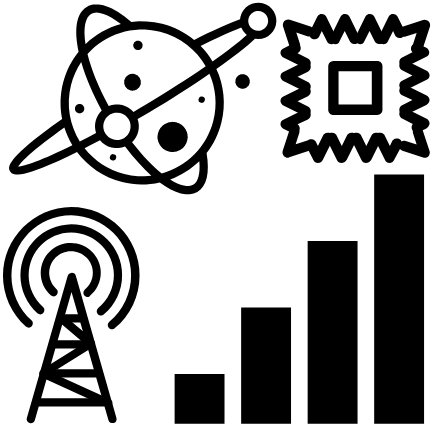
\includegraphics[width=0.14\paperwidth]{Images/logo_GB.png}%
		\vfill}
		}
}

% Set indentation
\setlength\parindent{0pt}

% Custom title commands
\titleformat{\section}
{\color{RED_SST}\normalfont\Large\bfseries}
{\color{RED_SST}\thesection.}{1em}{}
\titlespacing*{\section}
{0pt}{3.3ex}{3.3ex}

\titleformat{\subsection}
{\color{RED_SST}\normalfont\large\bfseries}
{\color{RED_SST}\thesubsection.}{1em}{}
\titlespacing*{\subsection}
{0pt}{3.3ex}{3.3ex}

% Custom headers and footers
\pagestyle{fancy}
\fancyhf{}
      
\fancyfoot{}
\fancyfoot[C]{\thepage} % page
\renewcommand{\headrulewidth}{0mm} % headrule width
\renewcommand{\footrulewidth}{0mm} % footrule width

\makeatletter
\patchcmd{\headrule}{\hrule}{\color{black}\hrule}{}{} % headrule
\patchcmd{\footrule}{\hrule}{\color{black}\hrule}{}{} % footrule
\makeatother

 
\renewcommand{\title}{Modulazione AM e Demodulazione di un segnale}
\renewcommand{\author}{Martina Coros}
\newcommand{\secondAuthor}{Samuele Verna}
\newcommand{\course}{Analisi ed Elaborazione dei Segnali}
\newcommand{\firstadvisor}{Prof. Fortunato SANTUCCI}
\newcommand{\secondadvisor}{Prof. Piergiuseppe DI MARCO}
\newcommand{\firstcoadvisor}{Dr. Graziano BATTISTI} % insert if any otherwise comment
\newcommand{\secondcoadvisor}{Dr. Graziano BATTISTI} % insert if any otherwise comment
\newcommand{\ID}{Matr. 111111}
\newcommand{\secondID}{Matr. 309996}
\newcommand{\YEAR}{2025-2026}

\renewcommand{\abstract}{In questo esperienza di laboratorio si è studiata la modulazione in ampiezza (AM) e la demodulazione di un segnale, processo fondamentale per la trasmissione dell'informazione in un contesto reale. Nel corso del laboratorio si sono realizzate tutte le fasi del processo, dalla generazione del segnale modulante alla modulazione del segnale portante, fino alla demodulazione del segnale ricevuto tramite l'utilizzo di un circuito e di un filtro. Durante l'esperimento sono state analizzate le caratteristiche dei segnali ottenuti tramite l'oscilloscopio. I risultati ottenuti hanno permesso di comprendere meglio i principi fondamentali del processo, nonché le applicazioni pratiche di queste tecniche nella trasmissione dei segnali.
}

\newcommand{\keywords}{Modulazione AM, Demodulazione, FFT, Filtro Passa-Banda, Teoria dei Segnali}

%-------------------------------------------------------------------------
%	BEGIN OF YOUR DOCUMENT
%-------------------------------------------------------------------------
\begin{document}

%-----------------------------------------------------------------------------
% TITLE PAGE
%-----------------------------------------------------------------------------
% DO NOT REMOVE SPACES BETWEEN LINES!

%\AddToShipoutPicture*{\BackgroundPic}
\begin{center}
    
\includegraphics[width=0.7\textwidth]{Images/logo_doppio.png}
\end{center}

\vspace{10mm}
\begin{center}
    \Large{\textbf{\color{RED_SST}{\title}}}\\
\end{center}

\vspace{4mm}
\begin{center}
    \fontsize{0.3cm}{0.5cm}\selectfont \bfseries \textsc{\color{RED_SST} Relazione attività Laboratorio SST  \\ \course}\\
\end{center}

\vspace{4mm}
\begin{center}
    \large{\textbf{\author, \ID}}

    \large{\textbf{\secondAuthor, \secondID}}
\end{center}

\small \normalfont

\vspace{11pt}

\centerline{\rule{1.0\textwidth}{0.4pt}}

\begin{center}
    \begin{minipage}[t]{.28\textwidth}
        \begin{minipage}{.90\textwidth}
            \noindent
            \scriptsize{\textbf{Advisors:}} \\
                \firstadvisor \\
                \secondadvisor \\
            \\
            \textbf{Co-advisor:} \\ 
                \firstcoadvisor \\ 
                %\secondcoadvisor \\ 
            \textbf{Academic year:} \\
                \YEAR \\
            \\
        \end{minipage}
    \end{minipage}
    \begin{minipage}{.70\textwidth}
        \noindent \textbf{\color{RED_SST} Sommario:} {\abstract}
    \end{minipage}
\end{center}

\vspace{15pt}

\begin{tcolorbox}[arc=0pt, boxrule=0pt, colback=RED_SST!60, width=\textwidth, colupper=white]
    \textbf{Key-words:} \keywords
\end{tcolorbox}

\vspace{12pt}

%%%%%%%%%%%%%%%%%%%%%%%%
%%      MAIN TEXT     %%
%%%%%%%%%%%%%%%%%%%%%%%%

%-----------------------------------------------------------------------------
% INDICE
%-----------------------------------------------------------------------------

\newpage
\tableofcontents
\newpage

%-----------------------------------------------------------------------------
% INTRODUCTION
%-----------------------------------------------------------------------------
\section{Introduzione}
\label{sec:Introduzione}

Questo è un file di esempio scritto in \LaTeX{}. Per creare una nuova sezione si possono usare i comandi:
\begin{verbatim}
\section{Titolo della sezione}
\label{sec:sezioneX}
\end{verbatim}
il primo per creare la sezione e il suo titolo mentre il secondo per creare una label ad esso per eventuali riferimenti nel testo. I riferimenti verranno fatti utilizzando il comando:
\begin{verbatim}
\ref{sec:sezioneX}
\end{verbatim}.

Analogamente si possono creare sottosezioni usando:
\begin{verbatim}
\subsection{Titolo della sottosezione}
\label{ssec:sottosezioneX}

\subsubsection{Titolo della sottosottosezione}
\label{sssec:sottosottosezioneX}
\end{verbatim}.

Volendo evitare la numerazione esplicita delle sezioni e sottosezioni si può usare il carattere "*" come segue:
\begin{verbatim}
\section*{Titolo della sezione}
\end{verbatim}


Per maggiori approfondimenti e dettagli su \LaTeX{} si può fare riferimento a \cite{oetiker1995not, kottwitz2015latex} oltre che allo svariato materiale presentein rete. 


%-----------------------------------------------------------------------------
% EQUATIONS
%-----------------------------------------------------------------------------
\section{Esempi di equazioni}
\label{sec:eqs}
Inseriamo qui un po' di esempi di equazioni varie tipo quelle di Maxwell:
\begin{subequations}
    \label{eq:maxwell}
    \begin{align}[left=\empheqlbrace]
    \nabla\cdot \bm{D} & = \rho, \label{eq:maxwell1} \\
    \nabla \times \bm{E} +  \frac{\partial \bm{B}}{\partial t} & = \bm{0}, \label{eq:maxwell2} \\
    \nabla\cdot \bm{B} & = 0, \label{eq:maxwell3} \\
    \nabla \times \bm{H} - \frac{\partial \bm{D}}{\partial t} &= \bm{J}. \label{eq:maxwell4}
    \end{align}
\end{subequations}

Del quale possiamo anche vederne il codice di seguito.

\begin{verbatim}
\begin{subequations}
    \label{eq:maxwell}
    \begin{align}[left=\empheqlbrace]
    \nabla\cdot \bm{D} & = \rho, \label{eq:maxwell1} \\
    \nabla \times \bm{E}+\frac{\partial \bm{B}}{\partial t} &=\bm{0}, \label{eq:maxwell2} \\
    \nabla\cdot \bm{B} & = 0, \label{eq:maxwell3} \\
    \nabla \times \bm{H} - \frac{\partial \bm{D}}{\partial t} &= \bm{J}. \label{eq:maxwell4}
    \end{align}
\end{subequations}
\end{verbatim}

La stessa si può fare anche con un singolo riferimento:
\begin{equation}
    \label{eq:maxwell_singlelabel}
    \left\{
    \begin{aligned}
    \nabla\cdot \bm{D} & = \rho, \\
    \nabla \times \bm{E} +  \frac{\partial \bm{B}}{\partial t} &= \bm{0},\\
    \nabla\cdot \bm{B} & = 0, \\
    \nabla \times \bm{H} - \frac{\partial \bm{D}}{\partial t} &= \bm{J}.
    \end{aligned}
    \right.
\end{equation}

\'E  possibile anche evitare i riferimenti alle equazioni come nelle seguenti:
$$
    Q(t)=C \cdot V \cdot (1-e^{-\frac{t}{RC}}) =C \cdot V \cdot (1-e^{-\frac{t}{\tau}})
$$

$$
    i(t)=\frac{V}{R} \cdot e^{-\frac{t}{\tau}}
$$

$$
    \int_{q_0}^{q} \frac{dq}{q} = -\int_{0}^{t} \frac{1}{R\cdot C}dt
$$

%-----------------------------------------------------------------------------
% FIGURES, TABLES AND ALGORITHMS
%-----------------------------------------------------------------------------
\section{Figure, Tabelle and Algoritmi}


\subsection{Figure}
\label{subsec:figures}

\begin{figure}
    \centering
        \begin{circuitikz}[scale=0.8]
        \draw (0,0)  node[above]{A} coordinate(in) to[R=\SI{15}{\kohm}, o-*] ++(3,0) coordinate(corner-in)
        to [C=\SI{10}{\uF}] ++(0,-2) % this -2 will fix the gnd line
        node[ground](GND){};
        \draw (in) to[open, v=$v_i(t)$] (in|-GND) node[ground]{};
        \draw (corner-in) -- ++(1,0) node[op amp, anchor=+](opamp){\texttt{LM358}};
        \draw (opamp.down) -- (opamp.down|-GND) node[ground]{};
        \draw (opamp.up) -- ++(0,1) to[crossing, name=X] ++(0,1) node[vcc]{\SI{5}{V}};
        \draw (opamp.-) -- ++(-1,0) |- (X.center)  -| (opamp.out);
        \draw (opamp.out) to[short, *-] ++(0.5,0) coordinate(rload)
        to[short, *-o] ++(1.5,0) coordinate(out) node[above]{B};
        \draw (rload) to[R=\SI{1}{\kohm}] (rload|-GND) node[ground]{};
        \draw (out) to[open, v^=$v_o(t)$] (out|-GND) node[ground]{};
\end{circuitikz}
    \caption{Circuito TikZ.}
    \label{fig:esempioCircuitoTikz}
\end{figure}

Per includere disegni e circuiti nel testo è possibile usare il pacchetto \texttt{TikZ} \cite{tikz} come in Figura~\ref{fig:esempioCircuitoTikz}, o includere un'immagine con il seguente comando:
\begin{verbatim}
\includegraphics[options]{filename.xxx}
\end{verbatim}
come in Figura~\ref{fig:esempioFigura1} e dove xxx è il formato, ad es. \verb|.png|, \verb|.jpg|, \verb|.eps|, \dots.

Anche qui esiste un ambiente particolare per inserire le immagine e i vari riferimenti usato per i riferimenti alla Figura~\ref{fig:esempioFigura1} o alle Figure~\ref{fig:EsempioUno}~e~\ref{fig:EsempioDue}.

\begin{figure}[H]
    \centering
    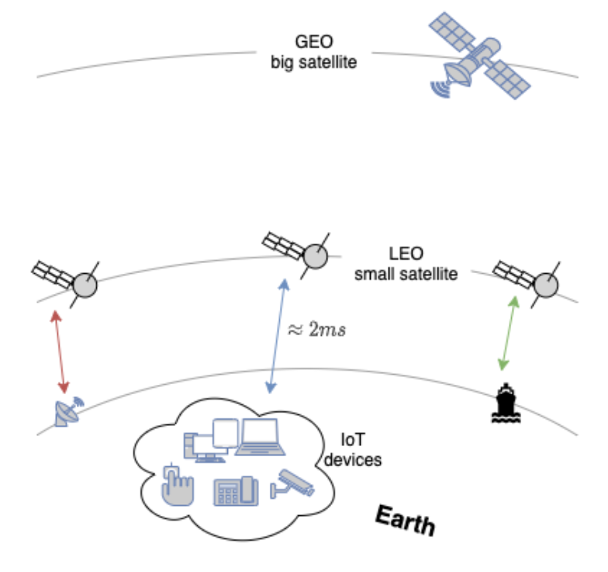
\includegraphics[width=0.5\textwidth]{Figure/Figura1.png}
    \caption{Prima figura di esempio.}
    \label{fig:esempioFigura1}
\end{figure}

\begin{figure}[H]
    \centering
    \subfloat[Esempio Uno.\label{fig:EsempioUno}]{
        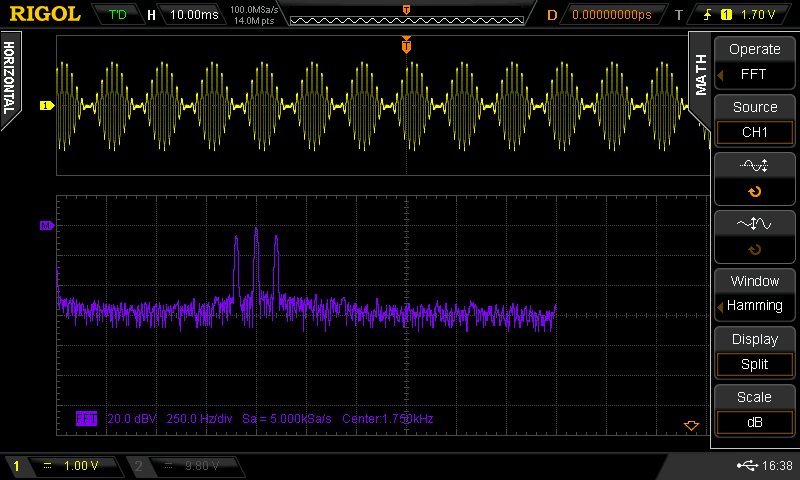
\includegraphics[width=0.45\textwidth]{Figure/Figura2.png}
    }
    \quad
    \subfloat[Esempio Due.\label{fig:EsempioDue}]{
        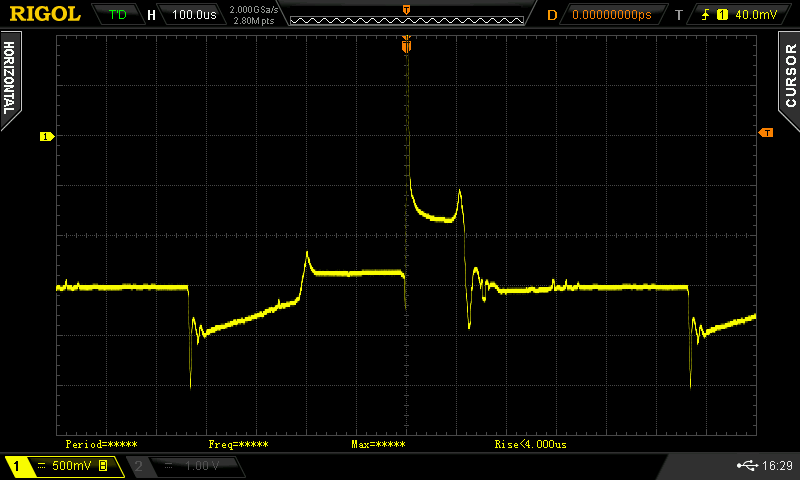
\includegraphics[width=0.45\textwidth]{Figure/Figura3.png}
    }
    \caption[]{Esempio composto.}
    \label{fig:quadtree2}
\end{figure}

\subsection{Tabelle}
\label{subsec:tabelle}

Un esempio di una tabella e del suo relativo ambiente in Tabella~\ref{table:EsempioColorato}.

\begin{table}[H]
    \caption*{\textbf{Titolo di Tabella}}
    \centering 
    \begin{tabular}{|p{3em}| c c c |}
    \hline
    \rowcolor{RED_SST!40}
     & \textbf{colonna 1} & \textbf{colonna 2} & \textbf{colonna 3} \T\B \\
    \hline \hline
    \textbf{riga 1} & 1 & 2 & 3 \T\B \\
    \textbf{riga 2} & $\alpha$ & $\beta$ & $\gamma$ \T\B\\
    \textbf{riga 3} & alpha & beta & gamma \B\\
    \hline
    \end{tabular}
    \\[10pt]
    \caption{Caption della tabella.}
    \label{table:EsempioColorato}
\end{table}



\subsection{Algorithm}
\label{subsec:Algorithm}

In \LaTeX si possono scrivere Pseudo-algorithms (o procedure esecutive) con i pacchetti \texttt{algorithm} e \texttt{algorithmic}.

Ottenendo qualcosa come nell'esempio dell'Algorithm~\ref{alg:var}.
\begin{algorithm}[H]
    \label{alg:example}
    \caption{Nome dell'algoritmo}
    \label{alg:var}
    \label{protocol1}
    \begin{algorithmic}[1]
        \STATE Initial instructions
        \FOR{$for-condition$}
            \STATE{Some instructions}
            \IF{$if-condition$}
                \STATE{Some other instructions}
            \ENDIF
        \ENDFOR
        \WHILE{$while-condition$}
            \STATE{Some further instructions}
        \ENDWHILE
        \STATE Final instructions
    \end{algorithmic}
\end{algorithm} 

\section{Ambienti di utilità generica}

Esistono svariati ambienti per i teoremi, corollari e loro dimostrazioni.

Elenchi puntati come i seguenti:
\begin{itemize}
    \item Primo 
        \begin{itemize}
            \item Caso A;
            \item Caso B.
        \end{itemize}
    \item Secondo
\end{itemize}
o numerati:
\begin{enumerate}
    \item Primo 
        \begin{enumerate}
            \item Caso A;
            \item Caso B.
        \end{enumerate}
    \item Secondo
\end{enumerate}

\section{Bibliography and citations}

Nel file \verb|bibliography.bib| ci sono tutti i riferimenti bibliografici utilizzati nel lavoro e questi vengoni utilizzati utilizzando il comando \verb|\cite{}|
\\

La bibliografia e la lista delle reference sono generate automaticamente dal programma  BibTeX \cite{bibtex}.

%-----------------------------------------------------------------------------
% CONCLUSION
%-----------------------------------------------------------------------------
\section{Conclusioni}
\color{black}
Qui vengono riportate le conclusioni principali dell'attività di ricerca o studio e i possibili sviluppi futuri.

%-----------------------------------------------------------------------------
% ACKNOWLEDGEMENTS
%-----------------------------------------------------------------------------
\section*{Acknowledgements}
Here you might want to acknowledge someone.


%-----------------------------------------------------------------------------
% BIBLIOGRAPHY
%-----------------------------------------------------------------------------
\bibliography{bibliography.bib}

\cleardoublepage


\appendix
\section{Appendice A\\ Strumentazione Utilizzata}

\subsection{Alimentatore}
\begin{figure}[H]
    \centering
    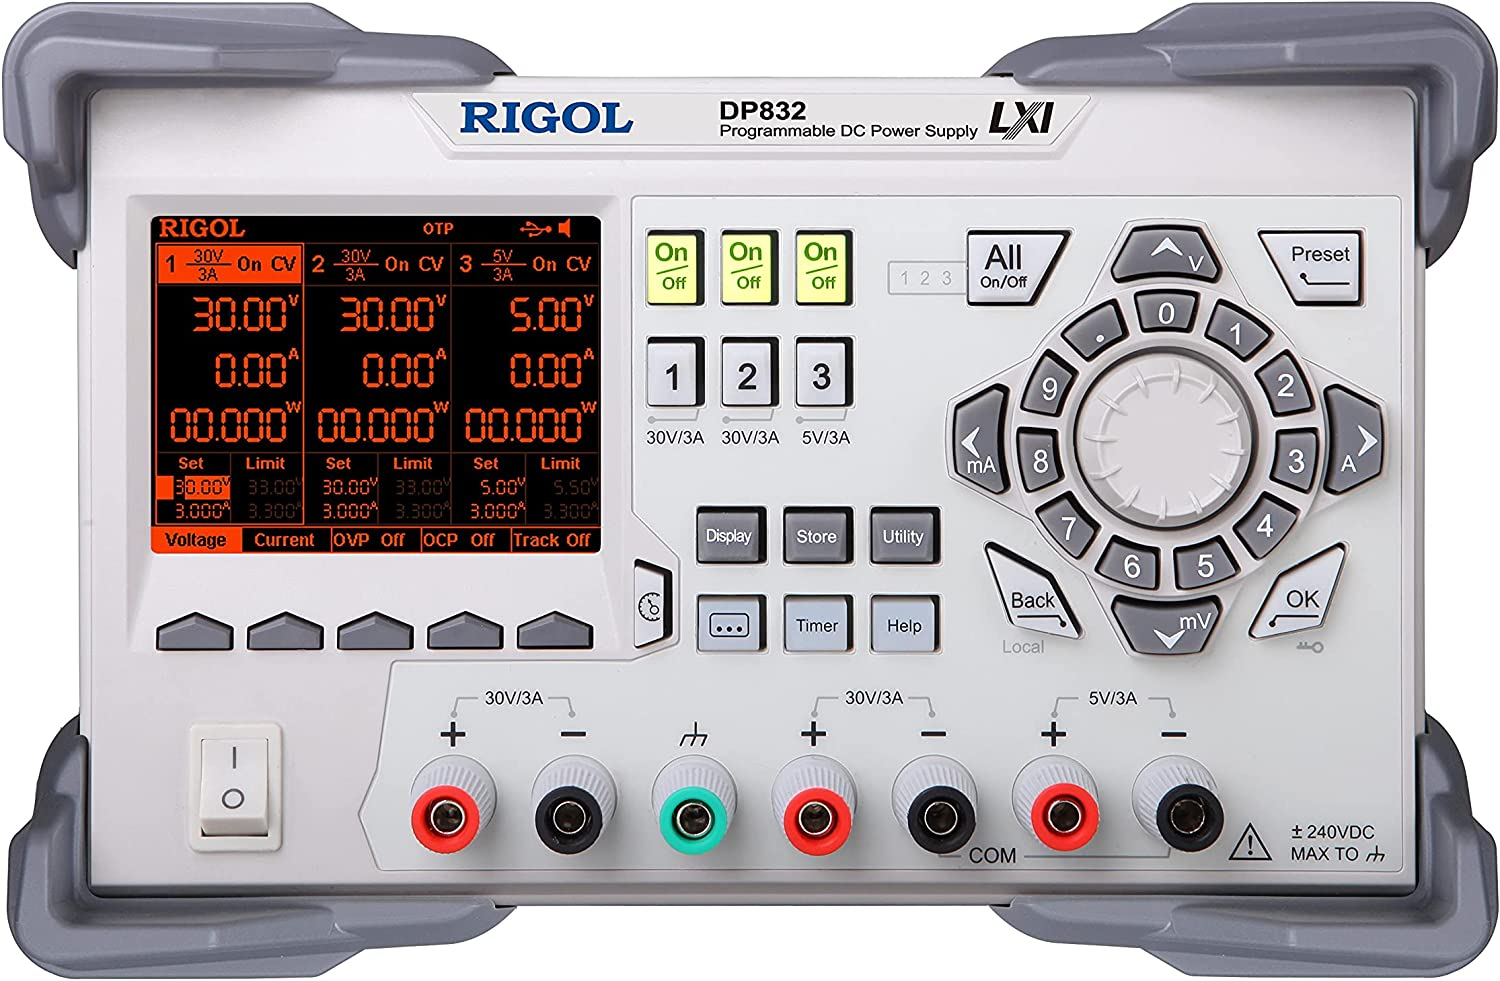
\includegraphics[width=0.5\textwidth]{Figure/Alimentatore.jpg}
    \caption{Alimentatore DP832 Rigol}
    \label{fig:Alimentatore}
\end{figure}

L'alimentatore è un importante strumento di laboratorio elettronico poiché consente ai ricercatori ed agli ingegneri di testare circuiti elettronici, dispositivi elettronici e componenti in modo sicuro e controllato, fornendo tensioni e correnti precise e regolabili.

Gli alimentatori possono essere a tensione fissa o variabile, e possono fornire corrente continua (DC) o alternata (AC), a seconda delle specifiche del dispositivo e dei requisiti dell'applicazione. Inoltre, gli alimentatori possono essere portatili o montati su rack a seconda dell'uso previsto.

Nel nostro laboratorio è presente l'alimentatore da banco a corrente continua portatile visibile in Figura~\ref{fig:Alimentatore}. Esso è costituito da 3 canali programmabili come segue:
\begin{itemize}
    \item {\bf CH1}: $\frac{30V}{3A}$ completamente indipendente;
    \item {\bf CH2}: $\frac{30V}{3A}$ negativo in comune con il CH3;
    \item {\bf CH3}: $\frac{5V}{3A}$ negativo in comune con il CH2;
\end{itemize}


\subsection{Multimetro}
\begin{figure}[H]
    \centering
    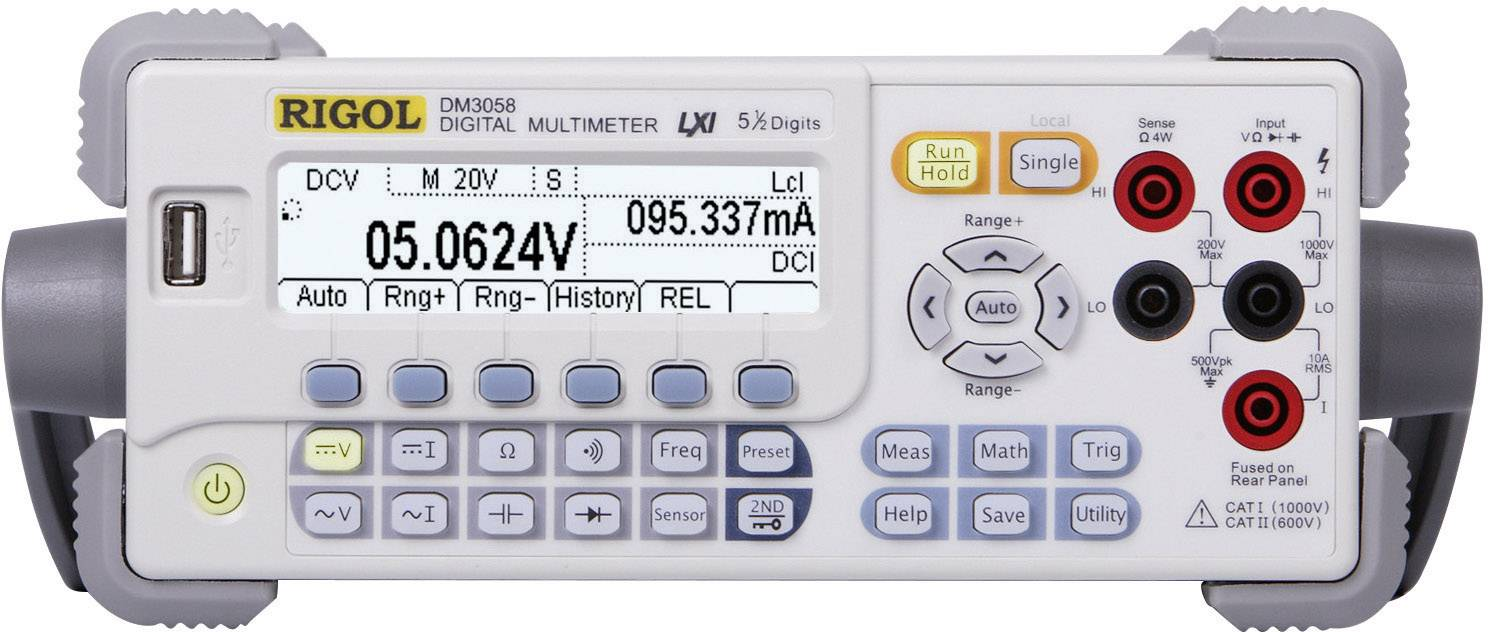
\includegraphics[width=0.5\textwidth]{Figure/Multimetro.jpg}
    \caption{Multimetro DM3058 Rigol.}
    \label{fig:Multimetro}
\end{figure}

Un multimetro (pronuncia multìmetro, conosciuto anche come multitester o semplicemente tester) è uno strumento di misura di grandezze elettriche che integra diverse funzioni, definite "campi di misura", in un'unica unità. Si presenta come una scatola dotata di una finestra di lettura (quadrante analogico a indice mobile oppure display digitale), uno o più comandi posti sul pannello frontale e almeno due boccole elettriche a cui collegare le sonde di misura (cavetti di diverso colore, terminanti con puntali ad impugnatura isolata)\cite{WIKIPEDIA-Multimetro}.

\subsection{Generatore di segnali}
\begin{figure}[H]
    \centering
    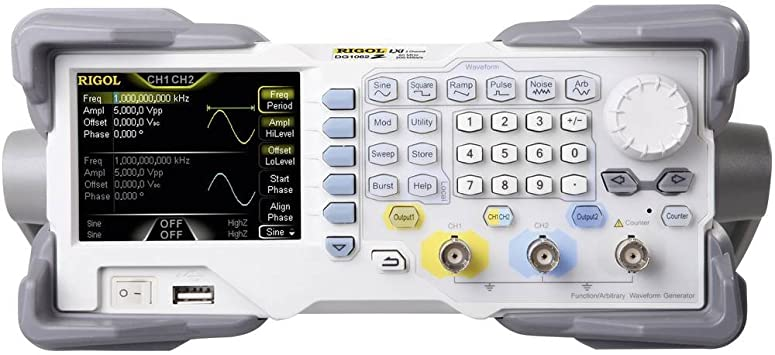
\includegraphics[width=0.5\textwidth]{Figure/GenSeg.jpg}
    \caption{Generatore di segnali DG1032Z Rigol.}
    \label{fig:GenSegnali}
\end{figure}

\subsection{Oscilloscopio}
\begin{figure}[H]
    \centering
    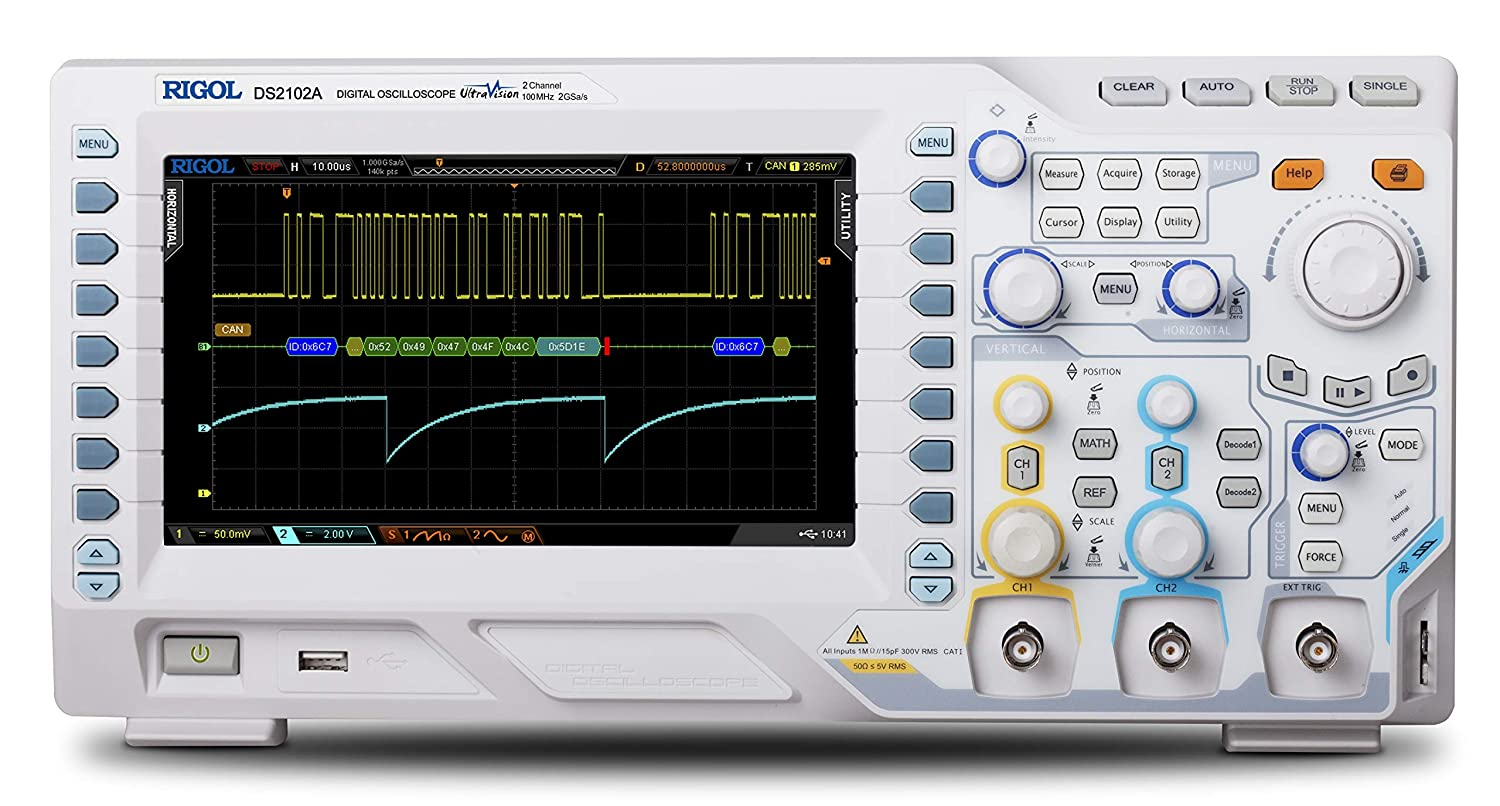
\includegraphics[width=0.5\textwidth]{Figure/Oscilloscopio.jpg}
    \caption{Oscilloscopio DS2102A Rigol.}
    \label{fig:Oscilloscopio}
\end{figure}


\pagebreak

\section{Appendix B\\ Corsi per la sicurezza effettuati}

Lo studente dichiara di aver effettuato tutti i corsi della sicurezza che consentono l'utilizzo dei laboratori in cui ha svolto la propria attività.

\begin{itemize}
    \item Corso Sicurezza base;
    \item Corso sicurezza specifico rischio basso;
    \item corso sicurezza specifico rischio medio.
\end{itemize}

\pagebreak

\section{Appendix C\\ Grafici in file esterni TikZ}

\subsection{Analisi di Fourier}


\begin{figure}[H]
    \centering
    \subfloat[Esempio Fourier 1.\label{fig:Fourier1}]{
        \input{Fourier}
    }
    \quad
    \subfloat[Esempio Fourier 2.\label{fig:Fourier2}]{
        \input{Fourier2}
    }
    \caption[]{Sviluppo di Fourier.}
    \label{fig:Fourier}
\end{figure}

\subsection{Disegni vari}

\begin{figure}[H]
    \centering
    \begin{tikzpicture}    %[nomestile/.style={opzioni}]
    %linee guida
    \draw [help lines] (-2.5,-2.5) grid (2.5,2.5);

    % Cambio posizione corrente
    \path (1,0);
    % \draw[opzioni] (coordinate pt iniziale)--(coordinate pt finale);
    \draw (-2.5,-2.5)--(2.5,2.5);

    %\node[opzioni] (label) at (coordinata pt) {testo}; 
    \node (origine) at(-1.5,0.5) {$\alpha$};
    \node at (1,1) {$\beta$};

    \draw (origine) -| ++(2,2) -| (origine);
    

\end{tikzpicture}

    \caption{Disegni vari TikZ.}
    \label{fig:DisegniVari}
\end{figure}

\subsection{Altro circuito}

\begin{figure}[H]
    \centering
    \begin{circuitikz}[scale=0.8]
       %\draw [help lines] (0,0) grid (5,5);

    \draw (2,4) node[pmos, bulk](M1){};
    \draw (2,1) node[nmos, bulk](M2){};

    \node[ground](GND) at (2,0) {};    
    \node[vcc](VCC) at (2,5) {\SI{5}{V}};
    
    \node[circ] (A) at (0,2.5) {};
    \node[circ] (B) at (2,2.5) {};
    \node[ocirc] (out) at (4,2.5) {};
    \node[ocirc] (in) at (-1,2.5) {};
    \draw (M1.S) to[short, *-] ++(1,0) |- (M1.bulk);
    \draw (M2.S) to[short, *-] ++(1,0) |- (M2.bulk);
    \draw (A) |- (M1.G);
    \draw (A) |- (M2.G);
    \draw (A) -- (in);    
    
    \draw (B) -- (M2.D);
    \draw (B) -- (M1.D);
    \draw (B) -- (out);
    

 %   \draw (A) to[short, *-o] (in);

    
    
\end{circuitikz}



    \caption{Altro esempio di circuito.}
    \label{fig:Circuito2}
\end{figure}

\subsection{Multirate}

\begin{figure}[H]
    \centering
    \begin{tikzpicture}[scale=1.8]
\begin{axis}[
    set layers=standard,
    domain=0:10,
    samples y=1,
    view={40}{20},
    hide axis,
    unit vector ratio*=1 2 1,
    xtick=\empty, ytick=\empty, ztick=\empty,
    clip=false
]

\draw [on layer=background, gray!20] (axis cs:0,2,0) -- (axis cs:0,8,0);
\pgfplotsinvokeforeach{1,2,3,4}{
    \draw (axis cs:0,#1*2,0) node[below, red]{$#1 \downarrow$} [on layer=background, gray!20]  -- (axis cs:10,#1*2,0) node[right, gray!80]{$t$};
    \addplot3 [on layer=main, blue!20, very thick, blue,ycomb,samples=256/2^#1]
      (x,#1*2,{1/2*sin(x*(75))+0.8*cos(x*(35)+20)});
}


\end{axis}
\end{tikzpicture}
    \caption{Multirate cambio di frequenza. Decimazione.}
    \label{fig:Multirate}
\end{figure}


\clearpage
\tableofcontents
%-------------------------------------------------------------------------
%	END OF YOUR DOCUMENT
%-------------------------------------------------------------------------
\end{document}